\documentclass{standalone}

\usepackage{xcolor}

\definecolor{myblue}{HTML}{377EB8}
\definecolor{myred}{HTML}{E41A1C}
\definecolor{myviolet}{HTML}{984EA3}
\definecolor{myteal}{HTML}{008B8B}

\usepackage{tikz}
\usepackage{pgfplots}
\pgfplotsset{compat=newest}

\usepackage{lmodern}
\SetSymbolFont{letters}{bold}{OML}{cmbr}{bx}{it}
\renewcommand{\familydefault}{\sfdefault}

\usepackage{sansmathfonts}

\begin{document}
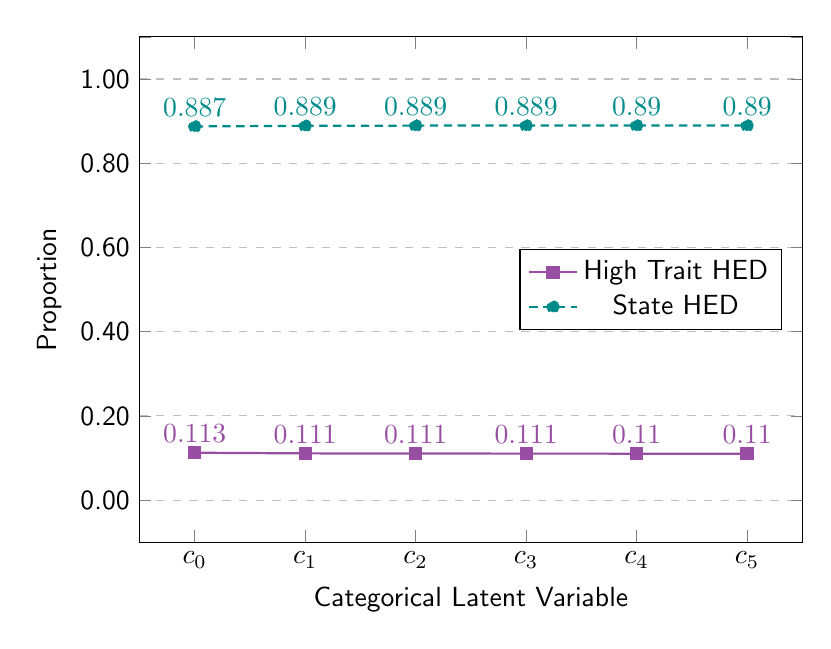
\begin{tikzpicture}
	\begin{axis}[
			xlabel={Categorical Latent Variable},
			ylabel={Proportion},
			ymin=-0.10,
			ymax=1.10,
			ytick={0.00,0.20,0.40,0.60,0.80,1.00,1.10},
			yticklabels={0.00,0.20,0.40,0.60,0.80,1.00},
			xtick=data,
			xticklabels={$c_{0}$, $c_{1}$, $c_{2}$, $c_{3}$, $c_{4}$, $c_{5}$},
			width=10cm,
			height=8cm,
			nodes near coords,
			nodes near coords={
				\pgfmathprintnumber[fixed, precision=3]{\pgfplotspointmeta}
			},
			legend style={at={(.97,0.5)},anchor=east},
			ymajorgrids=true,
			grid style=dashed,
		]
		\addplot[myviolet, mark=square*, solid, thick] coordinates {
			(1, 0.11262)
			(2, 0.11113)
			(3, 0.11066)
			(4, 0.11051)
			(5, 0.11046)
			(6, 0.11045)
		};
		\addplot[myteal, mark=oplus*, densely dashed, thick] coordinates {
			(1, 0.88738)
			(2, 0.88887)  
			(3, 0.88934)
			(4, 0.88949)
			(5, 0.88954)
			(6, 0.88955)
		};
		\legend{High Trait HED,State HED}
	\end{axis}
\end{tikzpicture}
\end{document}
